\chapter{Algorithm \todo{To be renamed?}}

Electron backscatter diffraction (EBSD) is a scientific tool used to examine crystalline materials. The principle of EBSD is sketched in \cref{ebsd-principle}. It is based on electron diffraction: when a beam of electrons is emitted towards the specimen, some of the electrons backscatter. They are then reflected on phosphor screen which is coupled with compact lens that directs the captured image towards a camera. The result of this procedure is a grayscale image of the \emph{electron backscatter pattern} (EBSP). An example of EBSP is shown in \cref{roi-shifts:initial}.

\begin{figure}
	\centering
	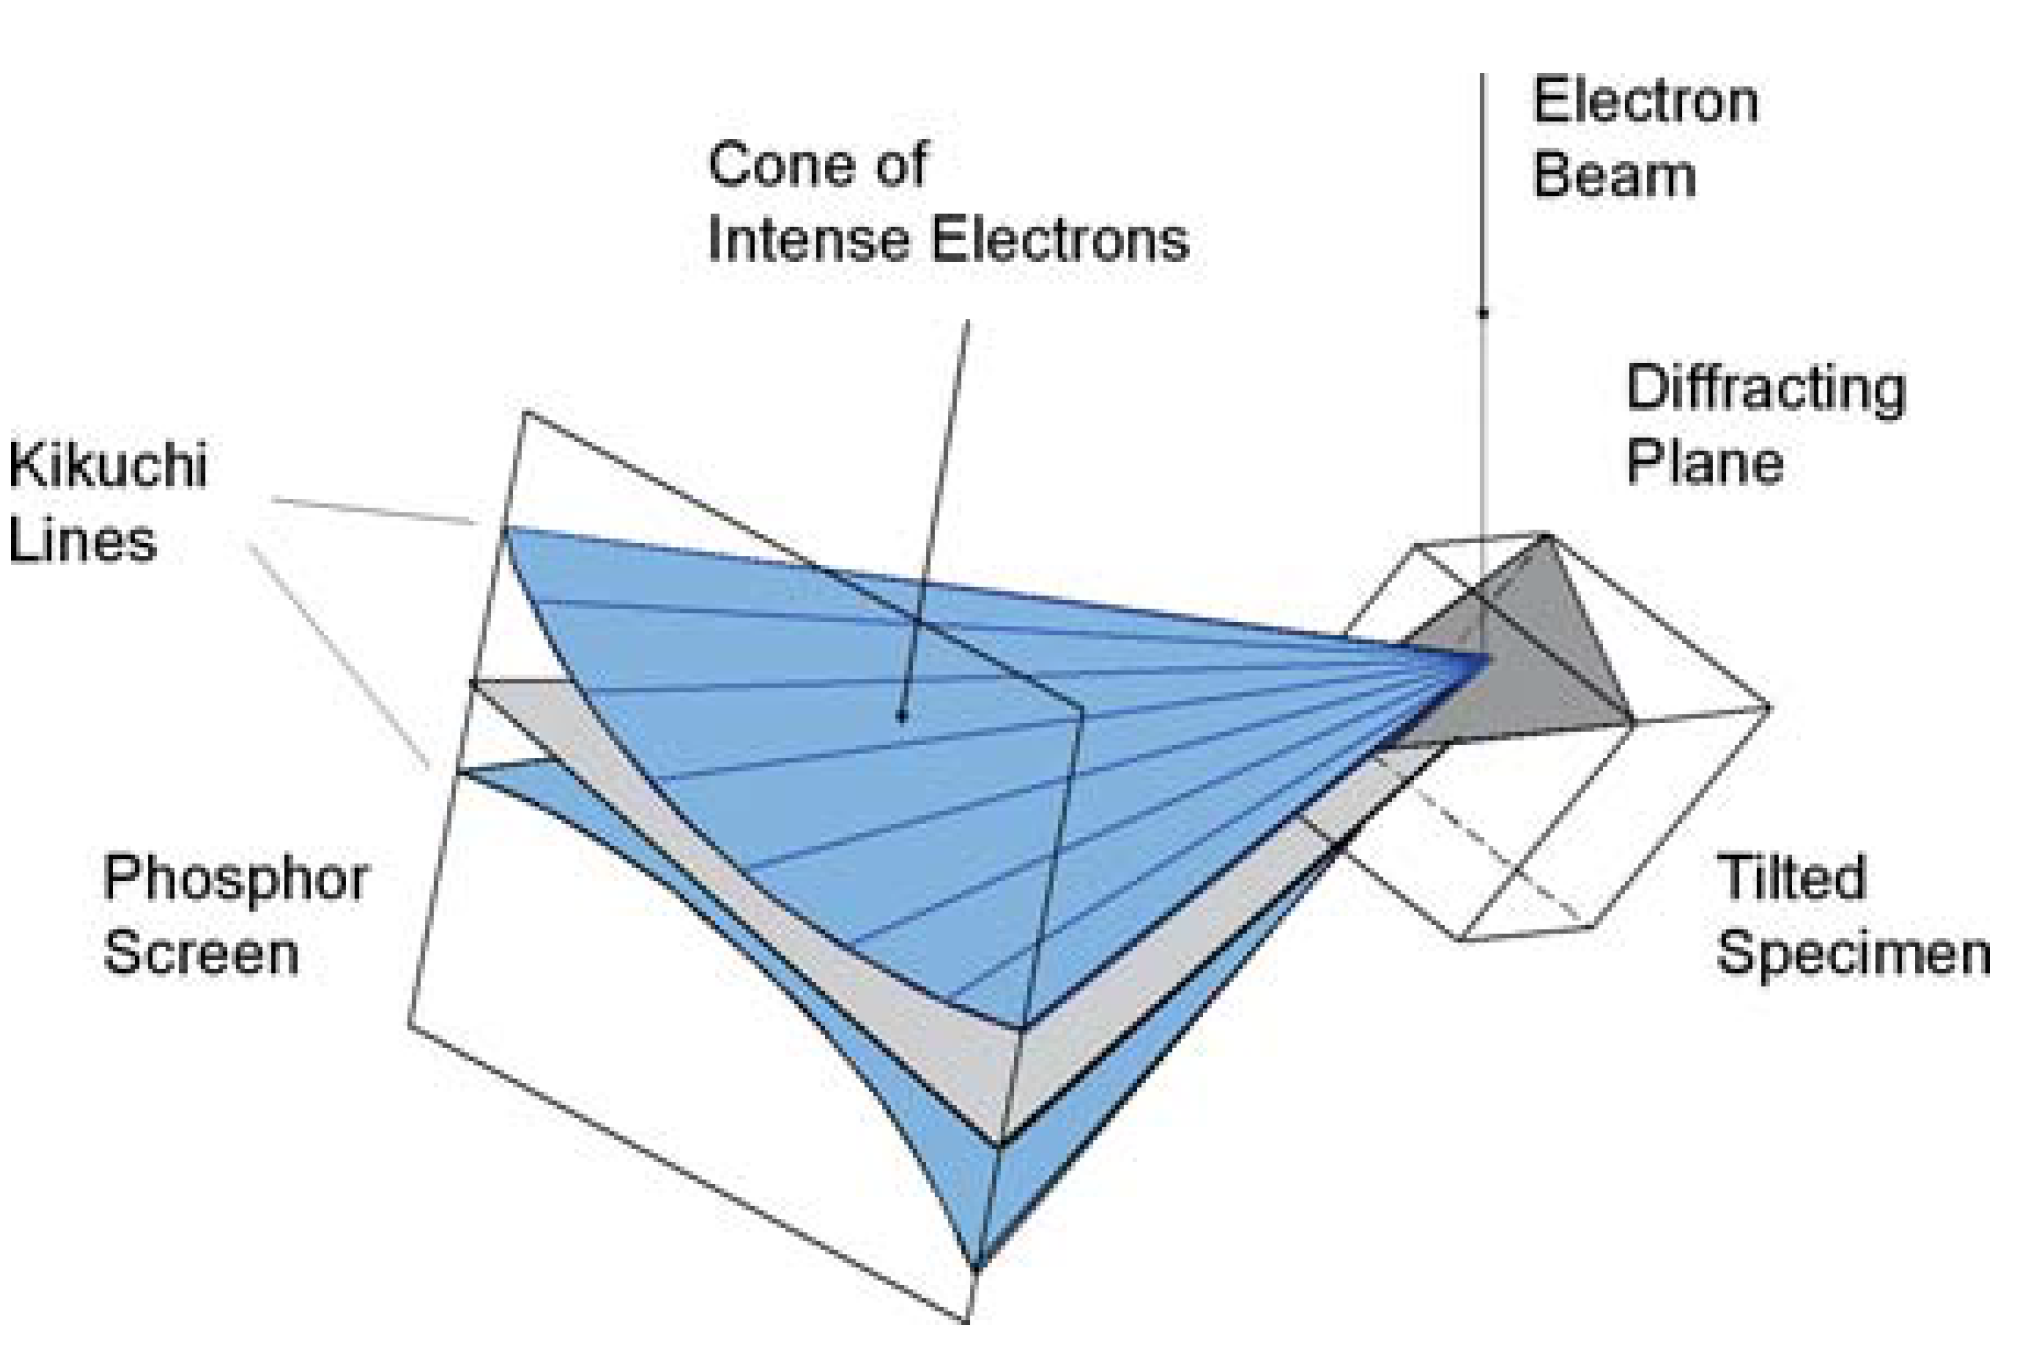
\includegraphics[width=0.7\textwidth]{img/ebsd_principle}
	\caption{The principle of EBSD. The image is taken from \cite{schwartz2009electron}.}
	\label{ebsd-principle}
\end{figure}

%\begin{figure}
%	\centering
%	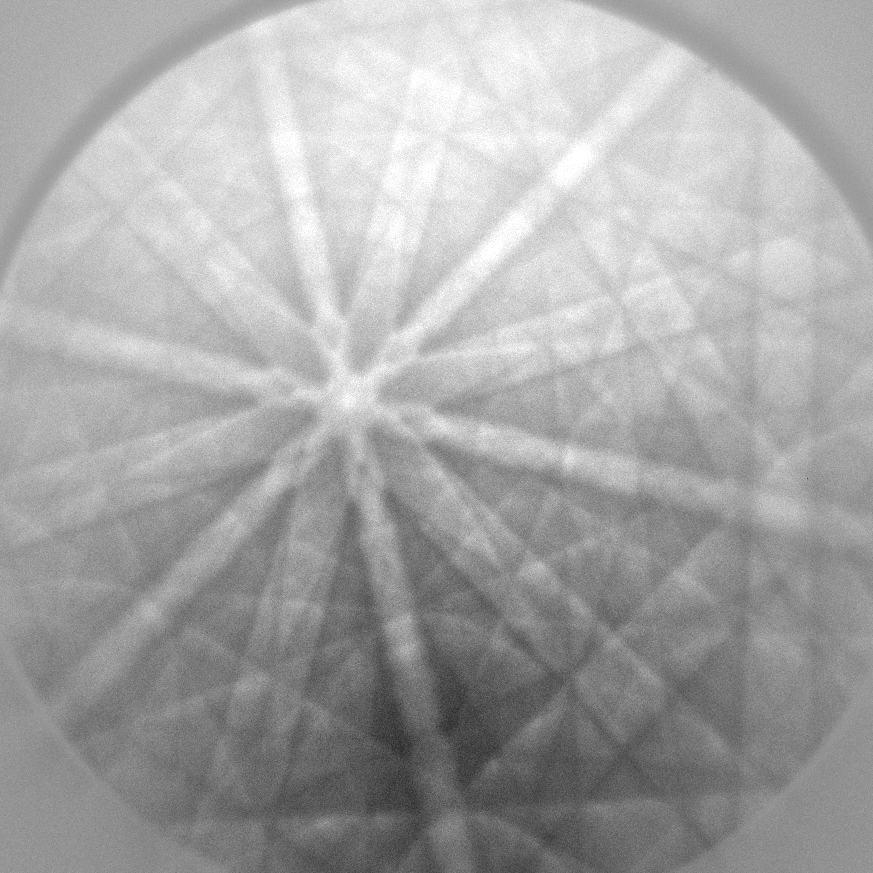
\includegraphics[width=0.7\textwidth]{img/INITIAL_x0y0}
%	\caption{Electron backscatter pattern of the FeAl compound.}
%	\label{ebsp-example}
%\end{figure}

The electrons do not reflect randomly, but based on the examined specimen, they backscatter in a specific way, forming \emph{Kukuchi lines} observable in the EBSP. The geometry of Kukuchi lines can be interpreted as a projection of the specimen crystal structure on the flat phosphor screen.

EBSD is commonly used with scanning electron microscopes (SEM). A SEM is a device that repeatedly emits an electron beam towards the specimen, scanning the surface in a raster pattern. That allows to create images of the surface of the sample with much greater magnification than light microscopes.

When used with EBSD, it creates the EBSPs in a raster scan pattern. It scans a part of the surface, measuring the crystalline structure of the specimen in many spots and saving the information as an EBSP. So the procedure results in thousands of images, one for each point in the raster. For example, test data that we used for this thesis contained over 15000 images taken from a 120x120 raster covering an area of the specimen surface approximately \SI{70}{\nano\meter}~x~\SI{70}{\nano\meter} big.

When the crystal structure of material is changed (e.g. under stress), the deformation can be observed in the EBSP too. Therefore, EBSPs of deformed specimen can be compared to undeformed ones to measure elastic strain and crystal lattice rotation.  \Cref{roi-shifts} shows a visualization of such comparison. Since different parts of the images may be deformed differently, a commonly used technique \cite{wilkinson2006high,wilkinson2010high,britton2012high} is to choose several (usually tens to hundreds) subregions of the EBSPs and determine the vector of shift between the corresponding regions from both patterns. The shifts estimate the real deformation of the crystalline structure.

\begin{figure}
	
	\begin{subfigure}{.5\textwidth}
		\centering
		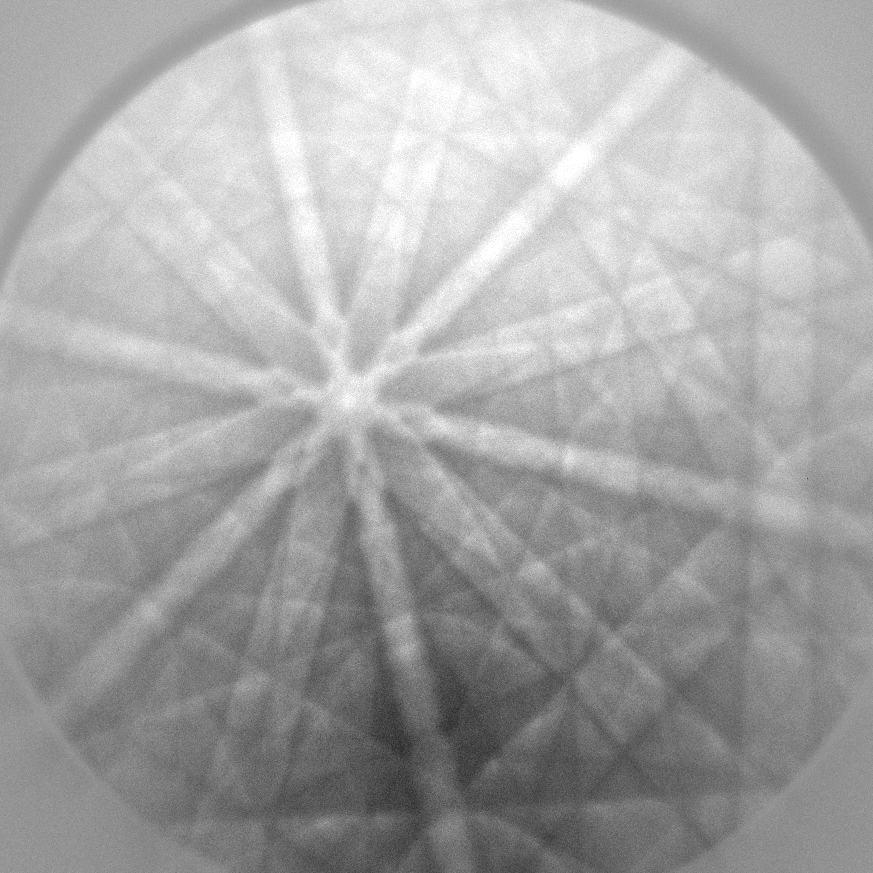
\includegraphics[width=.9\linewidth]{img/roi_shifts_initial}
		\caption{Initial, undeformed pattern}
		\label{roi-shifts:initial}
	\end{subfigure}%
	\begin{subfigure}{.5\textwidth}
		\centering
		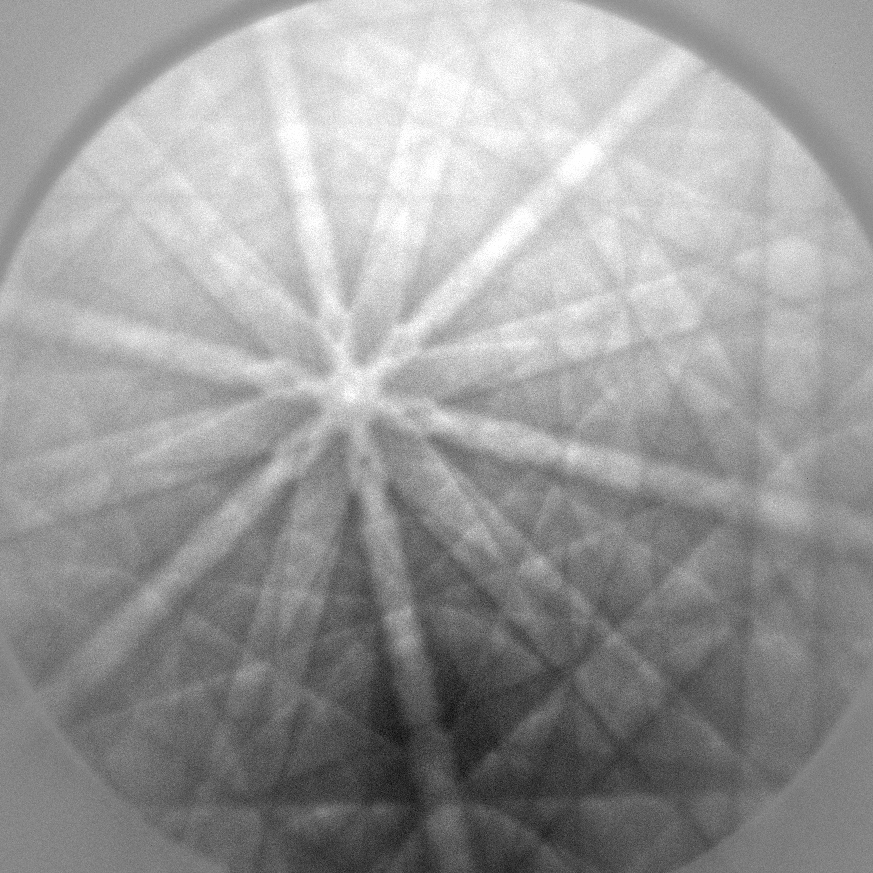
\includegraphics[width=.9\linewidth]{img/DEFORMED_x3600y6235}
		\caption{Deformed pattern}
		\label{fig:sub2}
	\end{subfigure}
	\centering
	\begin{subfigure}{.5\textwidth}
		\centering
		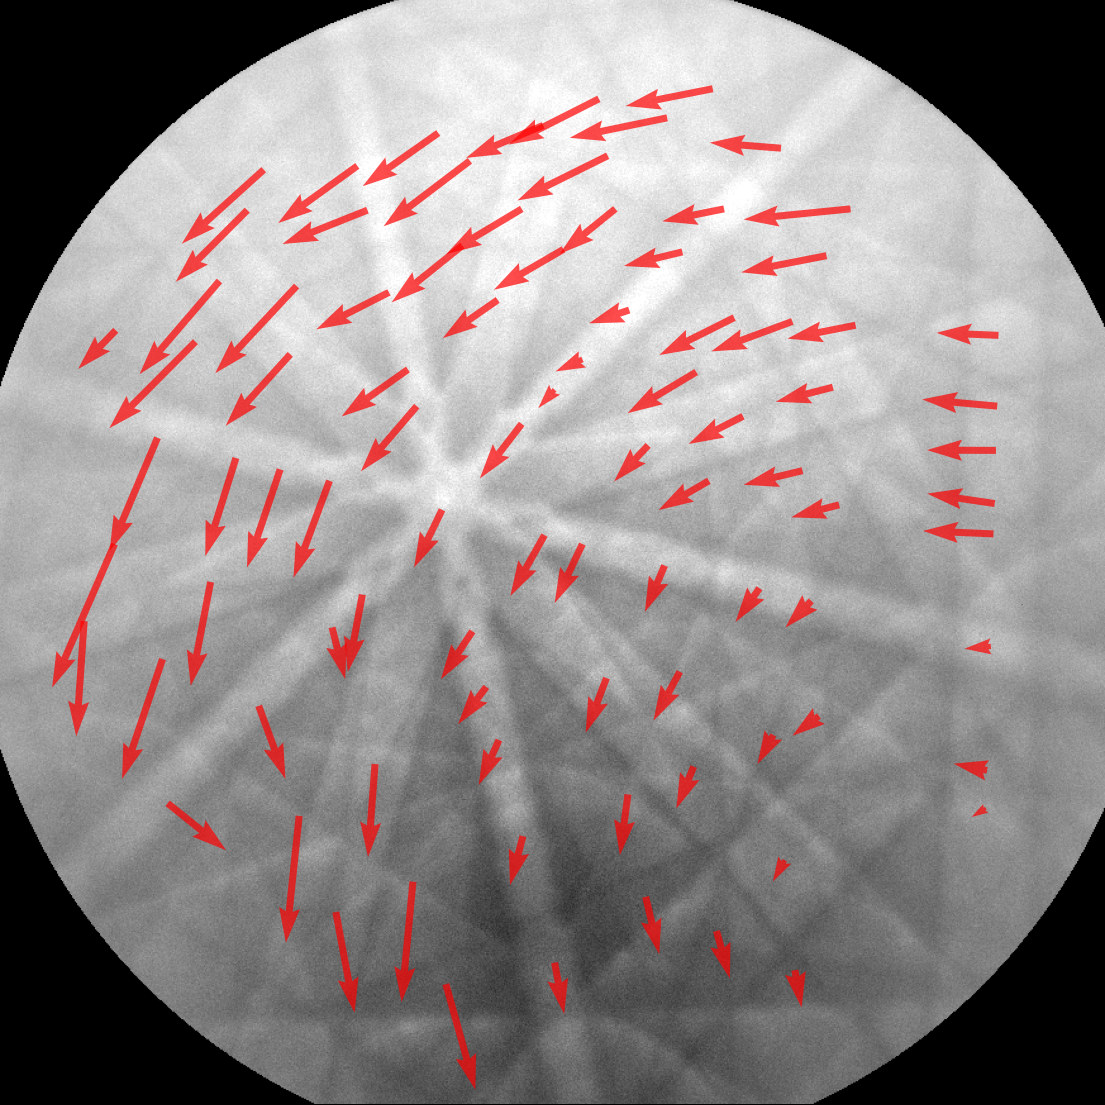
\includegraphics[width=.9\linewidth]{img/roi_shifts}
		\caption{Deformation visualization}
		\label{fig:sub2}
	\end{subfigure}

	\caption{Deformed pattern with arrows visualizing the deformation. The arrows are upscaled for the visualization, because the pattern is deformed only by several pixels (the biggest offset is less than 10 pixels long).}
	\label{roi-shifts}
\end{figure}

The comparison is done by cross correlating respective subregions of the deformed and reference EBSPs. The position of the maximum value in the correlation result determines the most probable shift with one pixel precision, which is not enough. To achieve subpixel accuracy, we estimate the peak of the cross correlation by interpolating from a small neighborhood of the maximum.

Once the shifts are computed, they are further processed to obtain an estimation of the actual crystal deformation and other characteristics. However, we do not address that part of the analysis in this thesis, as it is not nearly as computationally expensive as the cross correlation of the EBSPs. Moreover, the comparison is commonly used in analysis of EBSPs, while the processing of the shifts may be different for various purposes.

In this chapter we describe the technique based on cross correlation in detail.
\todo{summarize the chapter once it is done}

\section{Cross correlation}




\section{Algorithm description}

\begin{algorithm}[H]
	\KwIn{input}
	\KwData{this text}
	\KwResult{how to write algorithm with \LaTeX2e }
	initialization\;
	\ForEach{deformed EBSP}{
		load EBSP from disk\;
		\ForEach{ROI in EBSP}{
			cross correlate ROI from undefromed and deformed EBSP\;
			argmax\;
			subpixel peak\;
		}
	}
	\caption{How to write algorithms}
\end{algorithm}

Vstup:
Porovnavany obrazok
Obrazok predlohy
vyseky obrazku (nieco ako 32x32, parametrizovatelne)
I. cast
1. Pre kazdy vysek velkosti SxS: 
2. nacitat vyseky z oboch obrazkov,
3. vypocitat priemer pixelov
4. odpocitat priemer od oboch vysekov, aby sa hodnoty posunuli blizko k nule
5. aplikovat hanning (alebo iny) window na oba vyseky
6. cross-correlation - vysledkom je obrazok (2S-1)x(2S-1)
7. subpixel\_peak - je potrebne najst posunutie dvoch vysekov tak aby boli co najpodobnejsie.
8. najst maximalny pixel
10. zobrat okolie okolo neho a nafitovat hyperbolu metodou najmensich stvorcov
Vysledkom je zoznam posunuti jednotlivych vysekov

II. cast - z posunuti vypocitat vyslednu maticu zobrazenia.
Z vektorov spravne postavit maticu ktora zachycuje sustavu linearnych rovnic
vyriesit metodou najmensich stvorcov.

